% Chapter Template

\chapter{Results - Rubik's Cube} % Main chapter title

\label{sec:ResRubiks} % Change X to a consecutive number; for referencing this chapter elsewhere, use \ref{ChapterX}

%----------------------------------------------------------------------------------------
%	SECTION 1
%----------------------------------------------------------------------------------------





\begin{center}
\begin{tabular}{l*{5}{c}r}
\hline
\textbf{solver}      & & \textbf{Rubik's} & \textbf{2x2x2} & \textbf{3x3x3} \\
\hline
BFS   &   &        & x   &   \\
\hline
Kociemba   &   &      & x  &   \\
\hline
A$^{*}$[Kociemba]  &   &  & x & \\
\hline
A$^{*}$[DL[A$^{*}$[Kociemba]]]  &   &  & x & \\
\hline
A$^{*}$[DRL]  &   &  & x &  \\
\hline
A$^{*}$[DQL]  &   &  & x &  \\
\hline
MCTS[DQL][c=0]  &   &  & x &  \\
\hline
MCTS[DQL][c=69]  &   & & x &  \\
\hline
\end{tabular}
\end{center}








\Section{2x2x2}

1000 seq 30 shuffles training each target network update seen 1.1\% of all puzzles
199 of the 200 perfectly shuffled got solved well under 1h (median 83 seconds), only one outlier took about 67 minutes.


\begin{figure}[H]
\centering
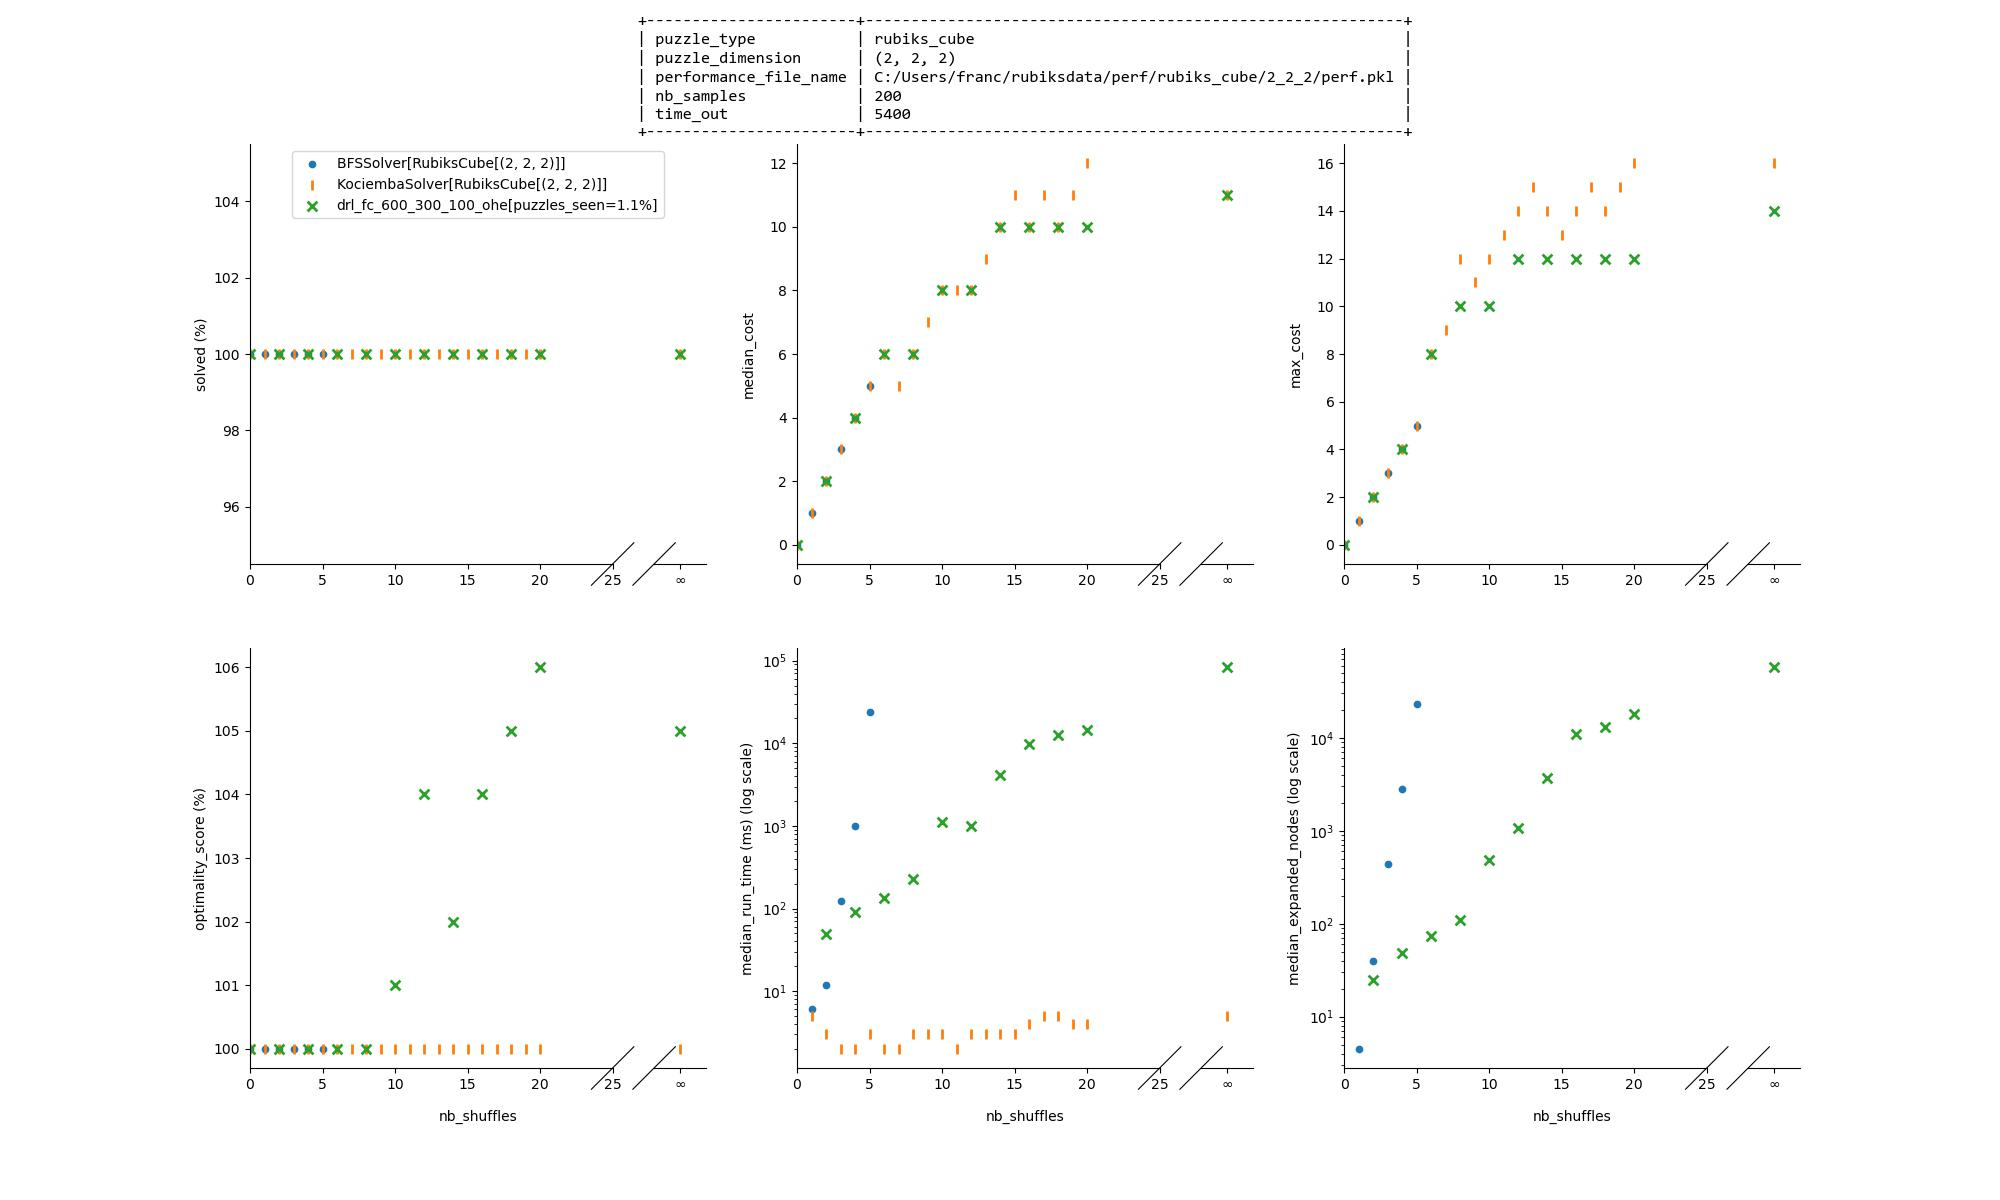
\includegraphics[scale=0.60]{./Figures/222RCPerformance}
%\decoRule
\caption[222RCPerformance]{Solvers' performance comparison 2x2x2 \textbf{RC}}
\label{fig:222RCPerformance}
\end{figure}



%-----------------------------------
%	SUBSECTION 1
%-----------------------------------
\Section{3x3x3}
\label{sec:ResRubiks333}

For now just showing Kociemba as a baseline. Will first try out DL trained on data generated from Kociemba, then will try out DRL. If unsuccessful or too slow, might try similar to paper using DQL/MC search.
\\
Notice Kociemba 3, unlike the 2x2x2 implementation that I found on github, does not do automatic color mapping. So if you present it with a cube which is not with the \textit{standard} centers (facing red and white up), it will actually not solve the cube. I have therefore added a bit of logic in Kociemba solver to look for the equivalent cube among the 24 equivalent cubes to the one being solved, with standard colors. We then solve this one using Kociemba and add the whole cube rotations to the solution (which in my code are deemed to have 0 cost anyway). This way, not only can I use Kociemba 3 to solve any (solvable) 3x3x3 cube irrespective of rotations, but I can also use that in A* or to train a DL network (also for A*)




\begin{figure}[H]
\centering
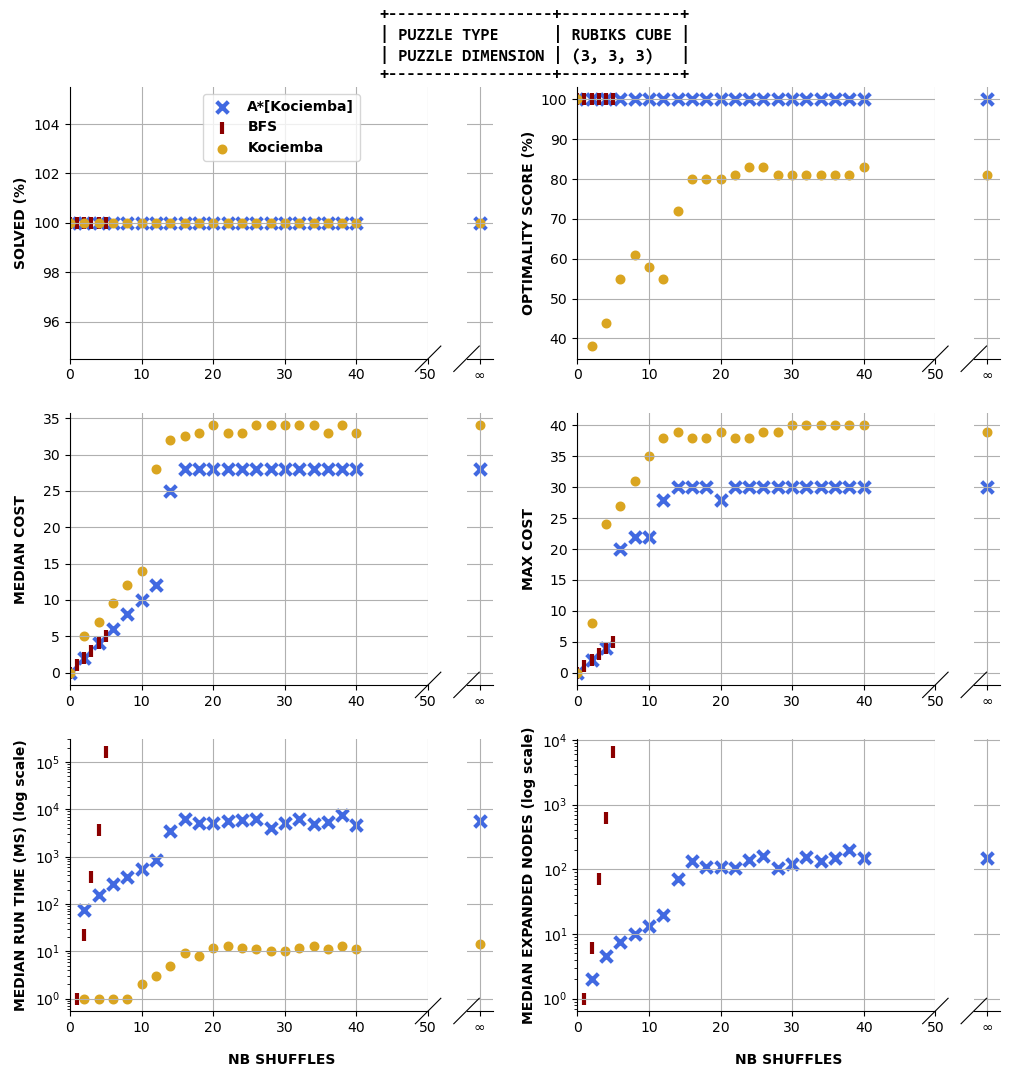
\includegraphics[scale=0.50]{./Figures/333RCPerformance}
%\decoRule
\caption[333RCPerformance]{Solvers' performance comparison 3x3x3 \textbf{RC}}
\label{fig:333RCPerformance}
\end{figure}
